\section{Application: the stochastic Allen--Cahn field}
\label{sec:allen-cahn}

\begin{figure*}[t]
  \centering
  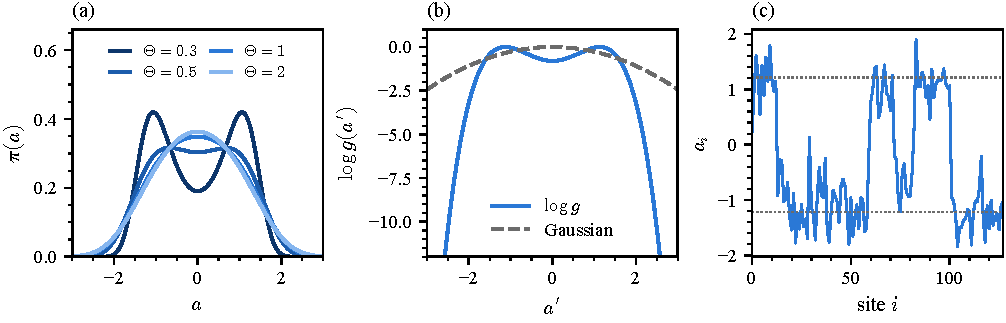
\includegraphics{fig_field}
  \caption{\note{(a) Single-site law at $\Theta=0.3$, $0.5$, $1$, $2$. (b) Kernel tilt $\log g$ against the Gaussian
  chain's quadratic. (c) One exact sample at $\Theta=0.3$; dotted: the wells.}}
  \label{fig:field}
\end{figure*}

\note{The application (12:01, 33:47). The SPDE $\partial_\tau\phi=\partial_x^2\phi-V'(\phi)+\sqrt{2\Theta}\eta$,
$V=\tfrac14(\phi^2-1)^2$; on a lattice its stationary law is a nearest-neighbour chain. Kernel = tilted walk
$\Normal(a';a,\gamma)g(a')$: the shape of the law of $a'$ depends on $a$. Cells: four $\Theta$, $L=32$, neighbour
correlation $0.85$ (E32).}

\begin{table}[t]
  \caption{\note{Error / best linear denoiser, $M=2048$, 16 seeds. Slide 15. Add the neural energy kernel row (E55).}}
  \label{tab:field}
  \centering
  \small
  \setlength{\tabcolsep}{4pt}
  \begin{tabular}{@{}lcccc@{}}
    \toprule
    $\Theta$ & 0.3 & 0.5 & 1 & 2\\
    \midrule
    site energy (5)          & 0.033 & 0.072 & 0.141 & 0.169\\
    tilted spline (25)       & 0.060 & 0.134 & 0.280 & 0.428\\
    log-linear 2-D (100)     & 0.184 & --    & 0.428 & --\\
    MDN (1{,}516)            & 0.228 & 0.422 & 0.738 & 0.838\\
    shift mixture (25)       & 1.004 & 1.004 & 1.014 & 1.021\\
    best network             & 0.484 & 1.174 & 2.157 & 3.044\\
    \bottomrule
  \end{tabular}
  % src: ~/Code/Thesis/jerome-call-2026-10-29-slide15.md (frozen E33 / E43 rows)
\end{table}

\note{J\'er\^ome's worry (38:50): at $\Theta=0.3$ the best network ($0.48$) beats the thesis kernel ($1.00$). Answer
from the frozen fits: the mixture is NOT collapsed (7.8 of 8 effective components); it is a shift family with linear
drift, so its best member is a Gaussian chain, and BP with it is linear. Every family whose law depends on $a$ beats
the best network in every cell, at $M=2048$ and $M=128$, including two with no field structure (log-linear 2-D $0.18$,
MDN $0.23$). Decide: keep the mixture row as the ``wrong family'' (as here) or drop it.}

\note{Data efficiency: with $M=128$ the site energy ($0.14$) beats the network with $2048$ ($0.48$). Parameter
recovery: $\hat\Theta/\Theta$ seed means $0.9995$--$1.0068$ (site energy, six cells, E33). Pending: E55, neural energy
kernel vs DDPM U-Net.}
